
\section{Related Work}
\label{sec:related}

%Modern analytics systems are usually built as a cluster of homogeneous machines
%networked using a fast interconnect. In such a configuration, the system can
%perform at its full potential if the dataset can fit in its collective DRAM.

In Big Data scale workloads, building a cluster with enough DRAM capacity to
accommodate the entire dataset can be very desirable but expensive. An example
of such a system is RAMCloud, which is a DRAM-based storage for large-scale
datacenter applications~\cite{ramcloud, rumble_log_dram}.  RAMCloud provides more than 64TBs of DRAM
storage distributed across over 1000 servers networked over high-speed
interconnect. Although RAMCloud provides 100 to 1000 times better performance
than disk-based systems of similar scale, its high energy consumption and high
price per GB limits its widespread use except for extremely performance and
latency-sensitive workloads.

NAND-Flash-based SSD devices are gaining traction as a faster alternative to
disks, and close the performance gap between DRAM and persistent storage.
SSDs are an order of magnitude cheaper price compared to DRAM,
and an order of magnitude faster performance compared to disk.
Many existing database and analytics software has shown
improved performance with SSDs~\cite{hadoopperf,ssdhadoop,ssddatabase}.
Several SSD-optimized analytics softwares, such as the SanDisk
Zetascale~\cite{zetascale} have demonstrated promising
performance while using SSD as the primary data storage.
Many commercial SSD devices have adopted high-performance PCIe interface in
order to overcome the slower SATA bus interface designed for
disk~\cite{fusionio, violinmemory, intelnvme}. Attempts to
use flash as a persistent DRAM alternative by plugging it into a RAM slot
are also being explored~\cite{diablotechnology}. 

SSD storage devices have been largely developed to be a faster drop-in
replacement for disk drives. This backwards compatibility has helped their 
widespread adoption.  However, additional software and hardware is required to
hide the difference in device characteristics~\cite{ssddesigntradeoff}.  Due to the high performance of
SSDs, even inefficiencies in the storage management software becomes
significant, and optimizing such software has been under active investigation.
Moneta~\cite{ucsd_moneta} modifies the operating system's storage management
components to reduce software overhead when accessing NVM storage devices.
Willow~\cite{ucsd_willow} provides an easy way to augment SSD controllers with
additional interface semantics that make better use of SSD characteristics, in
addition to a backwards compatible storage interface.  Attempts to remove the
translation layers and let the databse make high-level decisions~\cite{noftl}
have shown to be beneficial. 

Due to their high performance, SSDs also affect the network requirements.  The
latency to access disk over Ethernet was dominated by the disk seek latency.
However, in a SSD-based cluster the storage access latency could even be lower
than network access. These concerns are being addressed by faster network
fabrics such as 10GbE and Infiniband~\cite{infiniband}, and by low-overhead
software protocols such as RDMA~\cite{rdmampi, rdmahdfs, homrmapreduce, rdmahpc,
rdmampi, hadoopinfiniband} or user-level TCP stacks that bypass the operating
system~\cite{usertcp,userlevelprotocol}. QuickSAN~\cite{ucsd_quicksan} is an
attempt to remove a layer of software overhead by augmenting the storage device
with a low-latency NIC, so that remote storage access does not need to go
through a separate network software stack.

Another important attempt to accelerate SSD storage performance is in-store
processing, where some data analytics is offloaded to embedded processors inside
SSDs. These processors have extremely low-latency access to storage, and helped
overcome the limitations of the storage interface bus. The idea of in-store
processing itself is not new. Intelligent disks (IDISK) connected to
each other using serial networks have been proposed in 1998~\cite{idisk}, and
adding processor to disk heads to do simple filters have been suggested as early
as in the 1970s~\cite{searchprocessor,RAP,dbc}. However, performance improvements of such special
purpose hardware did not justify their cost at the time. 

In-store processing is seeing new light
with the advancement of fast flash technology. Devices such as Smart
SSDs~\cite{smartssdquery,smartssdcost,ucsd_willow} and Programmable
SSDs~\cite{xsd} have shown promising results, but gains are often limited by the performance of the embedded processors in such power constrained devices. 
Embedding reconfigurable hardware in storage devices is being
investigated as well. For example, Ibex~\cite{ibex} is a MySQL accelerator platform where a
SATA SSD is coupled with an FPGA. Relational operators such as selection and
group-by are performed on the FPGA whenever possible, otherwise they are
forwarded to software. Companies such as IBM/Netezza~\cite{netezza} offload operations such as filtering to a reconfigurable fabric near storage. On the other end of the spectrum, systems such as
XSD~\cite{xsd} embeds a GPU into a SSD controller, and demonstrates high
performance accelerating MapReduce.



Building specialized hardware for databases have been extensively studied and
productized. Companies such as Oracle~\cite{exadata} 
have used FPGAs to offload database queries.
FPGAs have been used to accelerate operations such as hash index
lookups~\cite{walkers}. Domain-specific processors for database queries are
being developed~\cite{databasefpga, hybridsql}, including Q100~\cite{q100} and LINQits~\cite{linqits}.
Q100 is a data-flow style processor with an instruction set architecture that
supports SQL queries. LINQits mapped a query language called LINQ to a set of
accelerated hardware templates on a heterogeneous SoC (FPGA + ARM). Both designs
exhibited order of magnitude performance gains at lower power, affirming that
specialized hardware for data processing is very advantageous.
However, unlike BlueDBM, these architectures accelerate computation on data that is in DRAM.
Accelerators have also been placed in-path between network and processor to perform operations
at wire speed~\cite{fpgastreamquery}, or to collect information such as
histogram tables without overhead~\cite{histogramssideeffect}.

%\begin{figure*}[t!]
%\centering
%\vspace{0pt}
%\begin{minipage}[c]{.4\paperwidth}
%\begin{center}
%	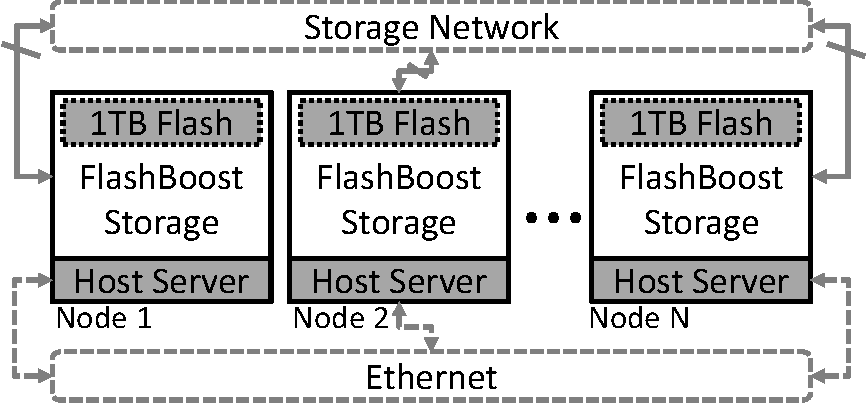
\includegraphics[width=\textwidth]{figures/architecture_small-crop.pdf}
%	\caption{BlueDBM Overall Architecture}
%	\label{fig:architecture}
%\end{center}
%\end{minipage}\hfill
%\vspace{0pt}
%\begin{minipage}[c]{.4\paperwidth}
%\begin{center}
%	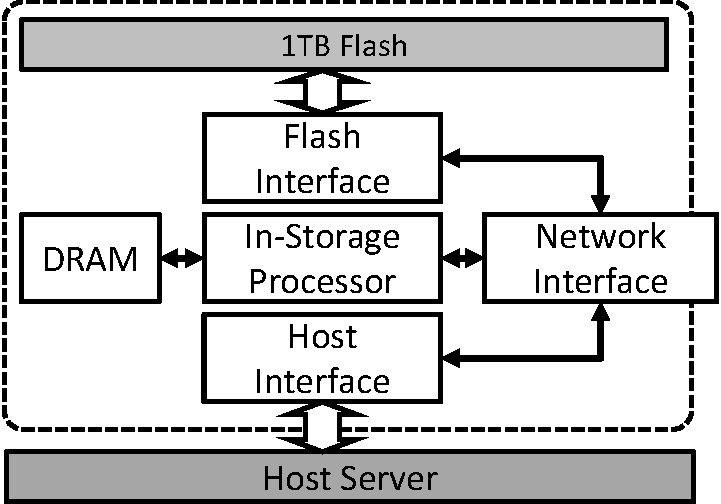
\includegraphics[width=0.7\textwidth]{figures/architecture_node-crop.pdf}
%	\caption{BlueDBM Node Architecture}
%	\label{fig:architecture_node}
%\end{center}
%\end{minipage}
%\end{figure*}



Incorporating reconfigurable hardware accelerators into large datacenters is also being investigated actively. Microsoft recently has built and
demonstrated the power/performance benefits of an FPGA-based system called
Catapult~\cite{msr_catapult}.  Catapult uses a large number of homogeneous
servers each augmented with an FPGA.  The FPGAs form a network among themselves
via high-speed serial links so that large jobs can be mapped to groups of FPGAs.
Catapult was demonstrated to deliver much faster performance while consuming
less power, compared to a normal ram cloud cluster. BlueDBM has similar
goals in terms of reconfigurable hardware acceleration, but it uses flash
devices to accelerate lower cost systems that do not have enough collective DRAM
to host the entire dataset.

%FIXME
This system improves upon our previous BlueDBM prototype~\cite{bluedbm}, which was a 4-node system with less than 100GB of slow flash. 
It was difficult to extrapolate the performance of real applications from the
results obtained from our previous prototype, because of both its size and
different relative performance of various system components. The current
generation of BlueDBM has been built with the explicit goal of running real applications, and will be freely available to the community for developing Big Data applications.

%The system closest in design to FlashBoost is BlueDBM~\cite{bluedbm}, but BlueDBM was a 4-node system with less than 100GB of slow flash. It is difficult to extrapolate the performance of real applications from the results obtained from BlueDBM, because of both its size and different relative performance of various system components. FlashBoost has been built with the explicit goal of running real applications, and will be freely available to the community for developing Big Data applications.

